\chapter{Introduction} \label{introduction} 

The purpose of this research is to make a contribution in the 
use of contextual information in recommender systems by proposing a methodology for
the development of context aware recommender systems.
The method includes an hybrid of several recommendation techniques and a
fuzzy inference system. The proposal was validated by 
the collection of contextual
information through questionnaires and the execution of several experiments,
with favorable results.

\section{Motivation}

Often people need take decisions, even if they do not
not have enought experience to decide among the possible alternatives. Often,
people trust the recommendations of friends or other people which they  
have certain level of affinity, when making decisions
according their personal interest.\\
As there is a large amount of information generated in a society, so, the
lack of experience of persons highlights the importance to provide
automatic methods to filter relevant information that helps to taking
desitions. \\Every day, a lot of information is generated in Internet
and it is available for users, then the overload information problem
arises, in a manner that users can't identify the relevant information
of the irrelevant. The users need tools to facilitate tasks, as well
as tools to provide a recommendation service that helps to use
efficiently the available information. The overload of information and
the lack of experience of users promotes the need of automatic search
engines that contributes to taking desitions through recommendations
of personalized products or services. \\ By other hand, in recent
years the mobile computing rocketed its importance because of the
impact of its use in daily life, any application can be applied in
mobiles and anywhere it can be used, their limitations are every time
less. For this reason, new technologies for use of context in mobile
applications arise, intelligent systems can take advantage of the
benefits that technology provides to manage the context that changing
constantly. Mobile and ubiquitous computing\cite{noguera2012mobile}
\cite{chiou2010adaptive} are proposing a wide variety of applications
that need recommendation engines using context for meet their
purposes.

\section{Context of use}\label{contextofuse}

Context is an important concept in everyday life. People often provide
context when writing postcards referring to the weather or holiday
atmosphere. A knowledge of context can also helps to explain why an
object was produced.\\  When a product (or system) is developed, it
will be used within a particular context. It will be used by a user
population with certain characteristics. The user will have certain
goals and wish to perform various tasks. The product will also be used
within a certain range of technical, physical and social or
organizational environments\cite{maguire2001context} that may affect
its use.\\   
We can refer to these environments as the \textit{context of use}(see
figure \ref{fig:logicalmodel}), this concept has been formally defined
by ISO standard 9241-11\cite{international1998iso} as \textit{``users,
tasks and equipment(hardware, software and materials), and the
physical and social environments in which a product is used"}. 
In the daily life we often finds products that are difficult to use or
understand. These types of difficults are \textit{usability problems}
that arise from  diverse issues that have not been addressed in the
design of the product's \textit{user-artefact interaction}. The
\textit{user-artefact interaction} refers the way that the user
interacts with the product and vice versa, this term has been studied
in Human Computer Interaction. \\As emerging technologies constantly
change the way people interact with products and their physical
environment, recent studies have started looking at \textit{human
experience} as a source to generate products or systems that
\textit{engage} the user.\\
The \textit{user experience}, \textit{context of use} and
\textit{product usability} have been associated in computer sciences
field. The \textit{Usability} is became a well-established concept in
the IT world to represent the user-friendliness of a system. However,
there was a need to establish the concept more clearly and to
determine how to measure it. Probably the best known definition of
usability is by Nielsen\cite{nielsen1994usability}: 
\textit{``usability is about learnability, efficiency, 
memorability, errors, and satisfaction".}
However, the definition of usability from ISO
9241-11\cite{international1998iso}:\textit{``the extent to which a
product can be used by specified users to achieve specified  goals
with effectiveness, efficiency and satisfaction in a  specified
context of use"}, is becoming the main reference of usability. \\
Thus, taking in account these definitions we can say that designing for 
\textit{usability} involves establishing user requirements for a new
\textit{system} or \textit{product}, developing design solutions,
prototyping the system and the user interface, and testing it with
representative users.\\
In the study of Sato\cite{sato2004context} that brings \textit{context
issues} into design practice, addressed the concept of
\textit{context} as a critical component of the design information in
order to enhance the \textit{human-centred design practice}. After a
literature's revision for  definitions of \textit{context} in diverse
fields, Sato explains that there are external and internal conditions
into the definitions and suggest that it has four characteristics:
\begin{enumerate}  
\item Aspects of context are based on the nature of actions and 
conditions.
\item Descriptions depends on the focus of the viewpoints.
\item Contextual changes are triggered from differents elements 
of the domain. 
\item Context evolves over the time, some aspects change fast
and others change slow. 
\end{enumerate} 
From this, Sato defined \textit{context} as a \textit{mental model} or a
\textit{pattern of one's memory} triggered by \textit{elements in the
situation}, where situation is a collective condition at the scene of
interaction composed of relations among \textit{variables of
conditions}. Sato employed this concept to describe the
\textit{influence of contexts} in \textit{people's interactions} and
\textit{system performance} and vice versa.\\
In this thesis we present the \textit{logical model} that explains how
the relation is among the concepts of \textit{context},
\textit{contextual information} and \textit{contextual factors}. The
figure \ref{fig:logicalmodel} represents in graphic mode the relations
between the concepts. The goal is to facilitate the use and
implementation of context in recommender systems for any application.\\
In the figure \ref{fig:logicalmodel}, the first box shows different
situations of the user (contexts), the user can changes from situation
to situation in a little time or a long time, this situational or
contextual information in the real world provides the knowledge that
the system needs to determine the context that will be used.  Next the
user context provides specific information found in his environment,
this we called \textit{``contextual factors"}(for instance, place and
orientation, preferences, date and time, etc.) and represents the
information that affects the recommendation process. The information
could be represents in fuzzy variables or crisp variables depending of
its domain values. Later, contextual factors are implemented as data
structures that define the domain proposed for each one. The number of
possible values varies for each application and is in this point where
the designers take desitions about the properly data structure  that
it'll be implemented.
%\begin{landscape} 
\begin{figure*}
\captionsetup{font=footnotesize} \centering
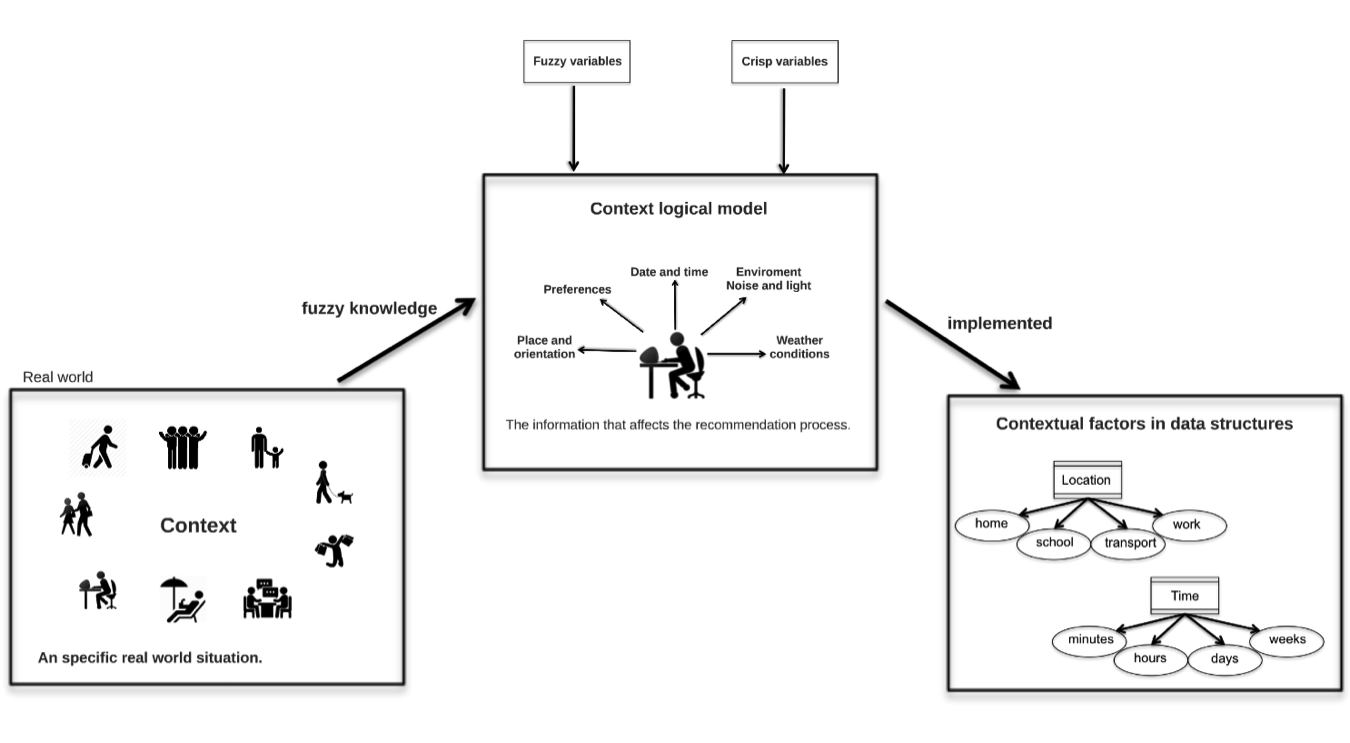
\includegraphics[width=1.0\textwidth]{img/context-scheme.png}  
\small
\caption{Logical data model of context for an application.}
\label{fig:logicalmodel}    
\end{figure*} %\end{landscape}

\section{Context-awareness} \label{context-awareness}

Traditional recommender systems provides suggestions of useful items
for a certain user. The suggestion relates to various decision-making
processes, for instance, what items to buy, what music to listen to or
what on-line news to read. \textit{Item} is the general term to denote
what product or service the system recommends for each user. A
recommender system normally focuses only in a type of item
\cite{resnick1997recommender}.
The improvements of previous recommender systems are focused in the
\textit{integration of context} in its recommendation process. 
The idea of \textit{context-aware computing} is to provide
information or services for the user based in the user's situation
\cite{dey2001understanding}. In order to do that, the application 
needs to obtain situational data, process it and make use of it 
in a manner that benefits the user. \\ 
\textit{Context} is a concept not easy to define, it is related with
several disciplines that propose different definitions. For example,
the authors Bazire et.al.\cite{bazire2005understanding} compare the
context in different fields and conclude that is complicated makes a
unifying definition of context because of the nature of the concept in
the disciplines. In computer sciences Fischer\cite{fischer2012context}
defines context as \textit{``the interaction between humans and
computers in socio-technical systems that takes place in a certain
context referring to the physical and social situation in which
computational devices and environments are embedded"}. Also identifies
the important aspects to consider when the context is used: how it is
the contextual data obtained, how the context is represented and what
goals and purposes the context has when is used in a particular
application. \\
Probably the definition most used in the field of recommender systems to 
define \textit{context} is proposed by Dey\cite{dey2001understanding}:
\textit{``Context is any information that can be used to characterize
the situation of an entity. An entity is a person, place or object
that is considered relevant to the interaction between a user and  an
application, including the user and applications themselves.''}  This
definition makes it easier to define the contextual factors in a
specific application. For instance, in a tourist guide application the
entities can be companion(friends, family, couple), place of interest,
season and weather, these could be considered as relevant contextual
factors that help the recommender system to provide items adjusted the
situational data of the user.\\
\textit{Context-aware recommender systems} are gaining even more
attention because of their performance and implementation for
different domains, the  way to improve personalized recommendations
based in contextual factors is an important technique to increase the
benefits in  many domains. For instance, taking in account the
\textit{hour of the day},  or the \textit{day of the week} when
recommending restaurants could  filter out restaurants that are
currently closed or near closing time, when the user receives this
information in real time, the user has the  way for taking
alternatives of restaurants that provide services. Nowadays, many
companies are incorporating some type of context (as time, location or
companion) in their recommendation engines, the application can be
found in fields such as e-commerce\cite{schafer1999recommender}
\cite{bulander2005enabling}, music\cite{ricci2012context}
\cite{baltrunas2011incarmusic} \cite{huq2010automated}, places of
interest\cite{baltrunas2012context},
movies\cite{eyjolfsdottir2010moviegen}, vacation
packages\cite{liu2011personalized} \cite{liu2014cocktail},  travel
guides\cite{savage2012m}, e-learning\cite{ortigosa2010entornos}  and
restaurants\cite{chu2013chinese}.\\
Plus, context can be used to improve the user satisfaction  in
recommender systems, thus the quality and accuracy of predictions  
is improved too. \\
The proposed method uses three recommendations techniques:
\begin{enumerate} 
\item \textit{Fuzzy Inference System}, this a rule based recommender
defined by an expert in the domain, it considers the following
variables: \textit{ratings average: low,medium and high},
\textit{price of restaurant: cheap, average and expensive}, and
\textit{number of ratings of item: few, several and many}, these
variables are used to infer how relevant a restaurant is for the user.
This recommendation is based on the popularity of each item in the
user community.
\item \textit{Content-based technique} utilizes the item profiles 
to compare how \textit{similar} is an item with respect to 
another, i.e. restaurants that are \textit{similar} (same cuisine, 
ambient, price range) to others that the user has rated high. 
The idea is to find items with similar features. 
\item \textit{Collaborative filtering technique} is based on the user
profile to identify user's preferences and to find neighbors that
have the same tastes. The recommendation consist in the suggestions of
other users with similar tastes that rated restaurants again in a
similar way but where have not been rated by the current user. A Top-N
list of restaurants is obtained to recommend for the user.
\end{enumerate} 
The results of the three techniques are a list of recommendations for
the user, later, these recommendations are adjusted in context. This
is the last step and is represented as \textit{context filter} in the
method, then the recommender system obtains a list of contextualized
recommendations. \\
In the method, each technique works simultaneously to obtain
recommendations, the hybrid method allows to generate suggestions even
without user information, i.e., using content-based technique or the
fuzzy inference system, so the system faces the cold-start or the
overspecialization problem using these thechniques, these problems are
described in section \ref{coldstart} and 
\ref{overspecialization}, respectively.\\
To test the performance were made several experiments that validate
the method, the algorithms were tested using contextual datasets and
the number of contextual factors used varies according the information
provided in the dataset. The goals of the experiments were to observe
the context role in the performance of the algorithms, what contextual
factors matter for users in a specific situation, how recommendations
are improved using context and, the accuracy in recommendations.
Chapter \ref{results} shows the results, discussion about results is
explained in each section.\\
Another important metric is the \textit{user satisfaction}, two
metrics were used to measure it: \textit{task-success} and \textit
{time-on-task}. These metrics allow to measure the user experience,
this offers so much more than just simple observation.\\ Usability
metrics can help reveal patterns that are hard or even impossible to
see. Evaluating software with a small sample size usually reveals the
most obvious usability problems\cite{albert2013measuring}.\\ Then, as
a general rule of thumb, during the early stages of design, it needs
fewer participants to identify the major usability issues. As the
design gets closer to completion, the tests should include more
participants to identify the remaining
issues\cite{albert2013measuring}.\\ 
Following this precept, ten representative users were selected to test
the system, subsequently, it was realized an analysis about the system
performance and issues presented in the user interaction. The chapter
\ref{evaluation} explains the process to evaluate the system and the
results obtained.
%%HECHO.

\section{Aims}

The contribution is to propose a method for context-aware recommender
systems using different techniques of recommendation, another aim is
to provide a \textit{useful knowledge} to utilize a hybrid method that
is easily implemented in different domains such as e-learning, movies,
music, tourism, etc. In this particular case, the restaurants domain
is used as a case of study to test the method.\\
Another important contribution is the use of fuzzy rules in the
proposed method, this allows the use of linguistic information closer
to the real context of the people, i.e., the method uses this
technique to analyze the user preferences and get recommendations
based in that information. For instance, the system provides a list of
range of prices, this allows the user to select a specific range of
price to get recommendations adjusted for the tag selected.\\ In order
to support the achievement of contributions, the particular aims of
this thesis are following:
\begin{itemize}  
\item Elaborate an analysis about state of the art in the field
of context-aware recommender systems through  the revision of
literature. 
\item Select the algorithms that represent alternatives of
solution for the problem in order to test their perfomance in different
domains.
\item Realize experiments with the proposed algorithms.
\item Based in previous experiments and results, to propose a hybrid
method and apply it in a case of study.
\item Define the fuzzy inference system that serves as recommender
technique in the proposed method, as well as the variables and fuzzy
rules involved.
\item Develop a prototype of context-aware recommender system 
using the proposed method.
\item To select the algorithms that represent alternatives of
solution for the problem to evaluate their perfomance in different
domains.
\item Evaluate the performance of the algorithms using 
different datasets in order to observe the system behaviour 
for each particular case.
\item Propose a hybrid method for context applied in a case of
study.
\item Develop a prototype of context-aware recommender system 
using the method in a specific domain.
\item Evaluate the proposed method using usability metrics.
\end{itemize} 

\section{Outline}

The rest of this thesis is organized as follows: 
\begin{itemize}  
\item \textbf{Chapter \ref{stateoftheart}} describes an in-depth study
of current background and related work is presented to give a general
overview of recommender systems and their evolution in recent years.
This study includes the traditional recommender systems, their methods
and techniques to improve recommendations, as so the problems to face
up this systems. Subsequently, the hybrid methods used in different
applications, their strenghts and weaknesses for each hibridation and
the domains of application. Finally, context-aware recommender systems
are mentioned, in the same way, we speak about the advantages and
disadvantages of the use of context in recommender systems.
\item \textbf{Chapter \ref{background}} describes the fundamental
concepts required to understand the proposed method.
\item \textbf{Chapter \ref{method}} presents a model of context-aware
recommender system, the proposed method  involves the paradigm of
post-filtering in a restaurants domain. This chapter include the
overall explanation of data models and  the method functionality, as
well as its components for this case of study.
\item \textbf{Chapter \ref{results}}, the general results of different
projects involved are presented along with the validation of every
experimentation. The experiments were realized using different
datasets and different algorithms in order to find an optimal manner
to reduce the error level. This chapter also details the results for
each experiment from a point of view of scientific results.
\item \textbf{Chapter \ref{evaluation}}, after the development of
context-aware recommender system, it was evaluated the impact of
context in recommendation process. This chapter describes the
usability tests that were applied on-line in order to evaluate the
satisfaction of users. Details of the environment and the
characteristics of the tests are described, as well as the results of
each one.
\item \textbf{Chapter \ref{conclusions}}, this chapter concludes with a
summary of its contributions and  its limitations. It discuss final
conclusions and the proposals for the future work.
\end{itemize}  

At the end, this thesis includes several appendices describing
detailed technical aspects of the context-aware recommender system
\textit{(appendix \ref{appendixc})}, the pseudocode of algorithms
\textit{(appendix \ref{appendixa})}, interfaces of the prototype of
context-aware recommender system \textit{(appendix \ref{appendixd})}
and experiment study materials \textit{(appendix \ref{appendixb})}.
